%    Latex Template for ACA 2016
%%%%%%%%%%%%%%%%%%%%%%%%%%%%%%%%%%%%%%%%
%    DO NOT CHANGE THE SETTINGS BELOW
%%%%%%%%%%%%%%%%%%%%%%%%%%%%%%%%%%%%%%%%
\documentclass[11pt]{article}
\usepackage{epsfig}
\usepackage{graphicx}
\usepackage[latin1]{inputenc}
\usepackage[T1]{fontenc}
\usepackage{mathptmx}
\usepackage{url}



\begin{document}



%%%%%%%%%%%%%%%%%%%%%%%%
%%%%%%%%%%%%%%%%%%%%%%%%%%%%%%%%%%%%%%%%
%    DO NOT CHANGE THE SETTINGS ABOVE
%%%%%%%%%%%%%%%%%%%%%%%%%%%%%%%%%%%%%%%%
%
\vspace{-0.8cm}
\begin{flushleft}
\Large \textbf{\noindent
%%% PLEASE INSERT THE TITLE OF YOUR TALK HERE %%%%%%%
Real-time animated dynamic geometry in the classrooms
by using fast Gr\"obner basis computations}
%%%%%%%%%%%%%%%%%%%%%%%%%%%%%%%%%%%%%%%%%%%%%%%%%%%%%%%%
\\
%%%%%%%%%%%%%%%%%%%%%%%%%%%%%%
\vspace{0.5cm}
\normalsize
 %%%%%%             NAMES OF AUTHORS         %%%%%%
 %%%%%% NAME OF SPEAKER SHOULD BE UNDERLINED %%%%%%%%%
\normalsize{
 %%%%%% FOR EXAMPLE %%%%%
 \underline{Z. Kov\'acs}$^1$
 %%%%%%%%%%%%%%%%%%%%%%%%
} \\
\vspace{5mm}
\textit{\footnotesize
 %%%%%% AFFILIATION OF AUTHORS %%%%%%
$^1$  The Private University College of Education of the Diocese of Linz, Austria,
zoltan@geogebra.org\\
 %%%%%%%%%%%%%%%%%%%%%%%%%%%%%%%%%%%%%
}
\end{flushleft}

The third millennium renaissance of elementary geometry by harnessing software applications in the classroom is already a history. By introducing dynamic geometry systems like \textit{The Geometer's Sketchpad}, \textit{Cabri} or \textit{Cinderella} the high number of mechanical numerical computations enabled students to make their own experiments with geometric objects easy.

Today's computers go one step forward. Not only fast numerical computations are available, but symbolical commands help, for instance, to expand or factorize expressions or solve equations or even equation systems.

Nevertheless, application of symbolic computations in dynamic geometry remained an unexplored field for many years. Recent researches in the direction to compute Gr\"obner bases significantly faster than earlier\footnote{See \cite{KP,K15} for two studies among the open source computer algebra systems.}, opened the road to manipulate on tens of equation systems in several variables within a second. Thus now it is possible to create real-time animations based on purely symbolic computations.
Such real-time animations include computing locus or envelope equations for geometry constructions on various software platforms like native Java programs, web applications or mobile/tablet solutions.

In this scientific work the state of the art will be demonstrated in the \textit{GeoGebra} dynamic mathematics tool which fully connects computer algebra and dynamic geometry. By computing and visualizing the algebraic equation of a non-trivial locus 29 frame per second (FPS) can be reached on an Intel(R) Core(TM) i7-2620M CPU @ 2.70GHz desktop computer (8 GB RAM installed, Ubuntu Linux 14.04.4). The same benchmark reaches 13 FPS as a web application in Google Chrome 49.0.2623.110.

Classroom application of the used technology is mainly on discovering general properties of geometry diagrams. GeoGebra---like many other DGS tools---makes it possible to construct a figure by using objects like points, lines or circles, and then, for example, GeoGebra's {\bf LocusEquation} command calculates the equation of a locus (given by the tracer and mover points) and plots that as an implicit curve. When the user drags the free points of the diagram, the locus equation will be automatically recomputed using heavy symbolic computations, but due to the effectivity of the calculations, the equation will be obtained very quickly. Finally the implicit curve will be plotted by using numerical methods, based on the symbolical form of the equation. (See \cite{K14} for a more detailed explanation.)

A similar scenario is to create the envelope equation of a set of output paths while the moving point is bound to another object. (An envelope is a curve that is tangent to each member of the family of the output paths at some point.) Obtaining the envelope is possible by using the {\bf Envelope} command in GeoGebra. More on this topic can be found in \cite{BR}.

Recently another form of the {\bf LocusEquation} command was introduced in GeoGebra, namely which calculates the locus of the free point such that a Boolean condition is satisified. This new form is also known as {\it implicit locus equation}. Due to the possibility to its direct use in the education, this third forms seems to be the most frequently used method to harness symbolic computations under the hood in a dynamic geometry experiment. For example, a natural way to discover Thales' theorem in the classroom is to construct a triangle $ABC$ with GeoGebra, and then type the command \texttt{LocusEquation[$a\perp b$,$C$]}. In this way the circle with diameter $AB$ will be immediately obtained and quickly redrawn when the free points $A$ or $B$ are dragged (Fig.~\ref{fig:Thales}).

\begin{figure}
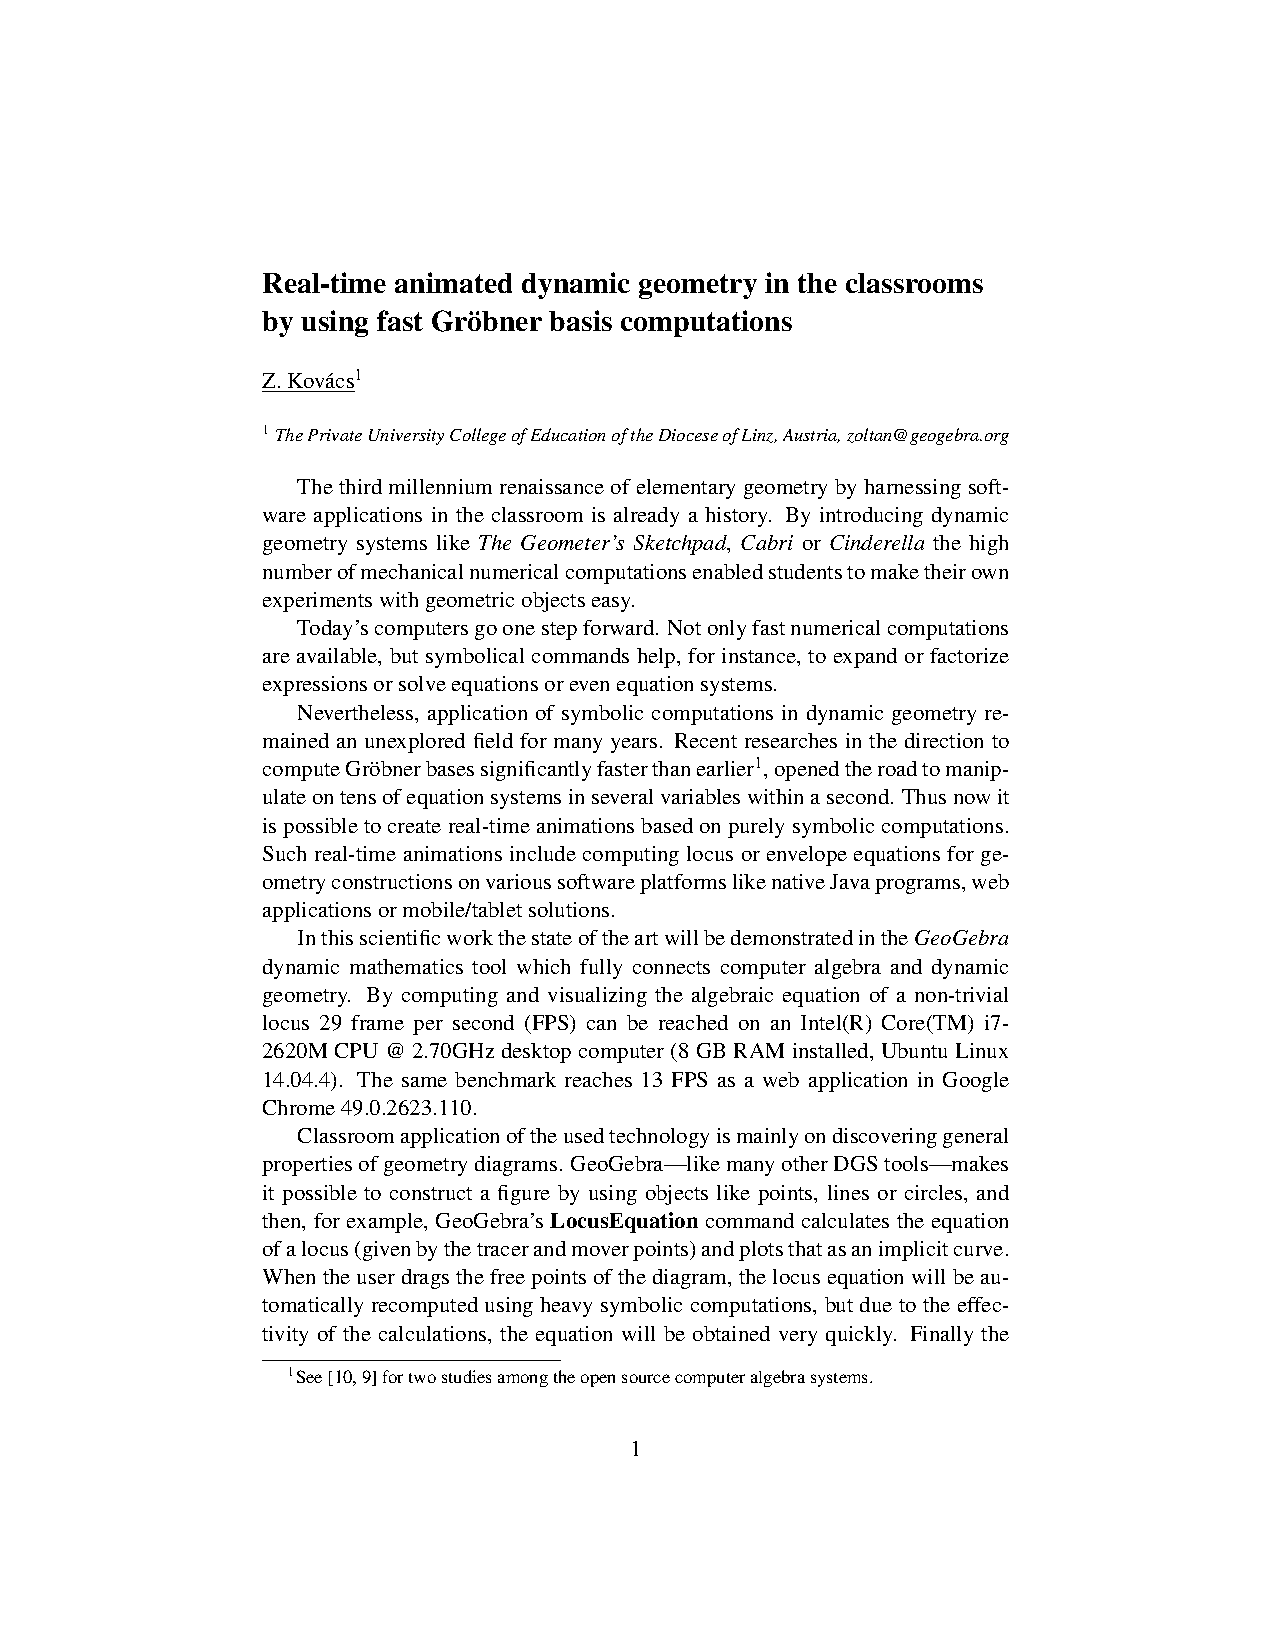
\includegraphics[width=\textwidth]{Kovacs}
\caption{An imaginary classroom discovery of Thales' theorem while dragging point $B$ from $(3,1)$ to $(4,3)$. Tracing is switched on for point $B$ and implicit curve $d$.
Here the animation reaches an average of 50 FPS for this simple theorem in desktop version of GeoGebra 5.0.237.0.}
\label{fig:Thales}
\end{figure}

All the three visualization activities above are common in using computational algebraic geometry to manipulate on coordinates of points, and their output is always an algebraic curve which is computed by---roughly speaking---eliminating some variables in the algebraic translation of the geometric construction. The elimination process is performed by the best available open source implementations, notably the standalone CAS \textit{Singular} and the embedded system \textit{Giac}.

The need to use symbolic computations instead of numerical ones in certain dynamic geometry visualization tasks is well discussed in the literature, see \cite{BK15}, section 3 for more details. All of the mentioned visualization activities are of the same kind.

The {\bf LocusEquation} command was introduced in 2010 in GeoGebra's development version by the pioneer work of Botana's, Ab\'anades', Escribano's and Arbeo's \cite{BK14,BK16}, to translate the geometric construction into an algebraic equation system. The elimination step was implemented by outsourcing the computations to the computer algebra system \textit{JAS} first, and later to \textit{Reduce}, Singular and recently to Giac \cite{KP}.
The visualization step of the locus equation as an implicit curve was implemented by Birklbauer and Drakuli\'c \cite{BD} in 2011.
Further improvements on the {\bf LocusEquation} command were based on the joint work of the pioneers, and Montes' and Recio's \cite{ABMR}.

Envelope support was added later by Botana and the author \cite{BK15} in 2013. Implementation of the implicit locus equation was achieved by Ab\'anades, Botana, Kov\'acs, Recio and S\'olyom-Gecse in 2016 (see \cite{ABKRS} for a collection of examples).

%%%%%%%%%%%%%%%%%%%%%%%%%%%%%%%%%%%%%%%


%%%%%%%%%%%%%%%%%%%%%%%%%%%%%%%%%%%%%%%%
%% BIBLIOGRAPHY
%%%%%%%%%%%%%%%%%%%%%%%%%%%%%%%%%%%%%%%%
\begin{thebibliography}{00}
\addcontentsline{toc}{chapter}{References}
\setlength{\itemsep}{-1mm}
\footnotesize

\bibitem{ABKRS} M. \'A. Ab\'anades, F. Botana, Z. Kov\'acs, T. Recio, C. S\'olyom-Gecse,
\textit{Implicit loci}, \url{http://tube.geogebra.org/m/mbXQuvUV} (2016).

\bibitem{ABMR} M. \'A. Ab\'anades, F. Botana, A. Montes, T. Recio, \textit{An algebraic taxonomy for locus computation in dynamic geometry}, Computer-Aided Design \textbf{56}, pp. 22-33
(2014).

\bibitem{BD} P. Birklbauer and D. Drakuli\'c, \textit{Implicit curves}. Second International GeoGebra Conference, Hagenberg, Austria.
\url{http://ggbconference2011.pbworks.com/w/file/fetch/44873718/presentation.pdf} (2011).

\bibitem{BK14} F. Botana and Z. Kov\'acs, \textit{Teaching loci and envelopes in GeoGebra},
\url{http://tube.geogebra.org/m/R8nUbEQV} (2014).

\bibitem{BK15} F. Botana and Z. Kov\'acs, \textit{A Singular web service for geometric computations},
Annals of Mathematics and Artificial Intelligence, \textbf{74}, 3, pp. 359-370 (2015).

\bibitem{BK16} F. Botana and Z. Kov\'acs, \textit{New tools in GeoGebra offering novel opportunities to teach loci and envelopes}.
\url{https://arxiv.org/abs/1605.09153}, arXiv:1605.09153 [cs.CG] (2016).

\bibitem{BR} F. Botana and T. Recio, \textit{Computing envelopes in dynamic geometry environments},
Annals of Mathematics and Artificial Intelligence, First online: 01 March 2016, pp. 1-18 (2016).

\bibitem{K14} Z. Kov\'acs, \textit{Loci problems in Age of Reason and their effect on GeoGebra -- Locus equations and their factorization in GeoGebra}. International GeoGebra Conference, Budapest, Hungary. \url{http://test.geogebra.org/~kovzol/talks/igi14/bp.pdf} (2014).

\bibitem{K15} Z. Kov\'acs, \textit{Computer based conjectures and proofs in teaching Euclidean geometry}. PhD thesis, Johannes Kepler University, Linz, Austria (2015).

\bibitem{KP} Z. Kov\'acs and B. Parisse, \textit{Giac and GeoGebra -- Improved Gr\"obner basis computations}, in \textit{Computer Algebra and Polynomials, Volume 8942 of the series Lecture Notes in Computer Science}, pp. 126-138 (2015). 

\end{thebibliography}
\normalsize
\end{document} 

